\documentclass[12pt]{beamer}
\usepackage{../Estilos/BeamerFC}
\usepackage{../Estilos/ColoresLatex}
\usepackage{courier}
\usepackage{listingsutf8}
\usepackage{listings}
\usepackage{xcolor}
\usepackage{textcomp}
\usepackage{color}
\definecolor{deepblue}{rgb}{0,0,0.5}
\definecolor{brown}{rgb}{0.59, 0.29, 0.0}
\definecolor{OliveGreen}{rgb}{0,0.25,0}
% \usepackage{minted}

\DeclareCaptionFont{white}{\color{white}}
\DeclareCaptionFormat{listing}{\colorbox{gray}{\parbox{0.98\textwidth}{#1#2#3}}}
\captionsetup[lstlisting]{format=listing,labelfont=white,textfont=white}
\renewcommand{\lstlistingname}{Código}


\definecolor{Code}{rgb}{0,0,0}
\definecolor{Keywords}{rgb}{255,0,0}
\definecolor{Strings}{rgb}{255,0,255}
\definecolor{Comments}{rgb}{0,0,255}
\definecolor{Numbers}{rgb}{255,128,0}

\makeatletter

\newif\iffirstchar\firstchartrue
\newif\ifstartedbyadigit
\newif\ifprecededbyequalsign

\newcommand\processletter
{%
  \ifnum\lst@mode=\lst@Pmode%
    \iffirstchar%
        \global\startedbyadigitfalse%
      \fi
      \global\firstcharfalse%
    \fi
}

\newcommand\processdigit
{%
  \ifnum\lst@mode=\lst@Pmode%
      \iffirstchar%
        \global\startedbyadigittrue%
      \fi
      \global\firstcharfalse%
  \fi
}

\lst@AddToHook{OutputOther}%
{%
  \lst@IfLastOtherOneOf{=}
    {\global\precededbyequalsigntrue}
    {}%
}

\lst@AddToHook{Output}%
{%
  \ifprecededbyequalsign%
      \ifstartedbyadigit%
        \def\lst@thestyle{\color{orange}}%
      \fi
    \fi
  \global\firstchartrue%
  \global\startedbyadigitfalse%
  \global\precededbyequalsignfalse%
}

\lstset{ 
language=Python,                % choose the language of the code
basicstyle=\footnotesize\ttfamily,       % the size of the fonts that are used for the code
numbers=left,                   % where to put the line-numbers
numberstyle=\scriptsize,      % the size of the fonts that are used for the line-numbers
stepnumber=1,                   % the step between two line-numbers. If it is 1 each line will be numbered
numbersep=5pt,                  % how far the line-numbers are from the code
backgroundcolor=\color{white},  % choose the background color. You must add \usepackage{color}
showspaces=false,               % show spaces adding particular underscores
showstringspaces=false,         % underline spaces within strings
showtabs=false,                 % show tabs within strings adding particular underscores
frame=single,   		% adds a frame around the code
tabsize=2,  		% sets default tabsize to 2 spaces
captionpos=t,   		% sets the caption-position to bottom
breaklines=true,    	% sets automatic line breaking
breakatwhitespace=false,    % sets if automatic breaks should only happen at whitespace
escapeinside={| |},  % if you want to add a comment within your code
stringstyle =\color{OliveGreen},
otherkeywords={as, np.array, np.concatenate, np.linspace, linspace, interpolate.interp1d, kind, plt.plot, .copy, np.arange, np.cos, np.pi, lw, ls, label, splrep, splev, plt.legend, loc, plt.title, plt.ylim, plt.show, sign, math.ceil, math.log, np.sqrt, np.exp, np.zeros, plt.xlabel, plt.ylabel, plt.xlim, np.identity, random, np.dot, np.outer, np.diagonal },             % Add keywords here
keywordstyle = \color{blue},
commentstyle = \color{darkcerulean},
identifierstyle = \color{black},
literate=%
         {á}{{\'a}}1
         {é}{{\'e}}1
         {í}{{\'i}}1
         {ó}{{\'o}}1
         {ú}{{\'u}}1
%
%keywordstyle=\ttb\color{deepblue}
%fancyvrb = true,
}

\lstdefinestyle{FormattedNumber}{%
    literate={0}{{\textcolor{red}{0}}}{1}%
             {1}{{\textcolor{red}{1}}}{1}%
             {2}{{\textcolor{red}{2}}}{1}%
             {3}{{\textcolor{red}{3}}}{1}%
             {4}{{\textcolor{red}{4}}}{1}%
             {5}{{\textcolor{red}{5}}}{1}%
             {6}{{\textcolor{red}{6}}}{1}%
             {7}{{\textcolor{red}{7}}}{1}%
             {8}{{\textcolor{red}{8}}}{1}%
             {9}{{\textcolor{red}{9}}}{1}%
             {.0}{{\textcolor{red}{.0}}}{2}% Following is to ensure that only periods
             {.1}{{\textcolor{red}{.1}}}{2}% followed by a digit are changed.
             {.2}{{\textcolor{red}{.2}}}{2}%
             {.3}{{\textcolor{red}{.3}}}{2}%
             {.4}{{\textcolor{red}{.4}}}{2}%
             {.5}{{\textcolor{red}{.5}}}{2}%
             {.6}{{\textcolor{red}{.6}}}{2}%
             {.7}{{\textcolor{red}{.7}}}{2}%
             {.8}{{\textcolor{red}{.8}}}{2}%
             {.9}{{\textcolor{red}{.9}}}{2}%
             {\ }{{ }}{1}% handle the space
         ,%
          %mathescape=true
          escapeinside={__}
          }



\usetheme{Warsaw}
\usecolortheme{seahorse}
%\useoutertheme{default}
\setbeamercovered{invisible}
% or whatever (possibly just delete it)
\setbeamertemplate{section in toc}[sections numbered]
\setbeamertemplate{subsection in toc}[subsections numbered]
\setbeamertemplate{subsection in toc}{\leavevmode\leftskip=3.2em\rlap{\hskip-2em\inserttocsectionnumber.\inserttocsubsectionnumber}\inserttocsubsection\par}
\setbeamercolor{section in toc}{fg=blue}
\setbeamercolor{subsection in toc}{fg=blue}
\setbeamercolor{frametitle}{fg=blue}
\setbeamertemplate{caption}[numbered]

\setbeamertemplate{footline}
\beamertemplatenavigationsymbolsempty
\setbeamertemplate{headline}{}


\makeatletter
\setbeamercolor{section in foot}{bg=gray!30, fg=black!90!orange}
\setbeamercolor{subsection in foot}{bg=blue!30}
\setbeamercolor{date in foot}{bg=black}
\setbeamertemplate{footline}
{
  \leavevmode%
  \hbox{%
  \begin{beamercolorbox}[wd=.333333\paperwidth,ht=2.25ex,dp=1ex,center]{section in foot}%
    \usebeamerfont{section in foot} \insertsection
  \end{beamercolorbox}%
  \begin{beamercolorbox}[wd=.333333\paperwidth,ht=2.25ex,dp=1ex,center]{subsection in foot}%
    \usebeamerfont{subsection in foot}  \insertsubsection
  \end{beamercolorbox}%
  \begin{beamercolorbox}[wd=.333333\paperwidth,ht=2.25ex,dp=1ex,right]{date in head/foot}%
    \usebeamerfont{date in head/foot} \insertshortdate{} \hspace*{2em}
    \insertframenumber{} / \inserttotalframenumber \hspace*{2ex} 
  \end{beamercolorbox}}%
  \vskip0pt%
}
\makeatother

\makeatletter
\patchcmd{\beamer@sectionintoc}{\vskip1.5em}{\vskip0.8em}{}{}
\makeatother

%\newlength{\depthofsumsign}
%\setlength{\depthofsumsign}{\depthof{$\sum$}}
% \newcommand{\nsum}[1][1.4]{% only for \displaystyle
%     \mathop{%
%         \raisebox
%             {-#1\depthofsumsign+1\depthofsumsign}
%             {\scalebox
%                 {#1}
%                 {$\displaystyle\sum$}%
%             }
%     }
% }
\def\scaleint#1{\vcenter{\hbox{\scaleto[3ex]{\displaystyle\int}{#1}}}}
\def\scaleoint#1{\vcenter{\hbox{\scaleto[3ex]{\displaystyle\oint}{#1}}}}
\def\bs{\mkern-12mu}

\usefonttheme{serif}

\title{Tema 0 - Introducción a python 1}
\author{M. en C. Gustavo Contreras Mayén}
\date{16 de agosto de 2023}

\fontsize{14}{14}\selectfont
\spanishdecimal{.}

\begin{document}
\maketitle

\section*{Contenido}
\frame[allowframebreaks]{\tableofcontents[currentsection, hideallsubsections]}

\section{Uso del equipo en aula}
\frame{\tableofcontents[currentsection, hideothersubsections]}
\subsection{Claves de acceso}

\begin{frame}
\frametitle{Al encender el equipo}
Se usará la distrubución de Fedora (linux), una vez cargado el inicio, hay que seleccionar el siguiente usuario:
\end{frame}
\begin{frame}
\frametitle{Usuario de trabajo}
Usuario: \textbf{est5}
\\
\bigskip
\pause
Contraseña: \textbf{est536WMM}
\end{frame}
\begin{frame}
\frametitle{El equipo en sesión}
Una vez que ya tengamos la sesión abierta, manejaremos algunos comandos básicos de linux para nuestro próposito.
\end{frame}
\begin{frame}
\frametitle{Abriendo Anaconda}
Para lanzar Anaconda, hay dos opciones:
\pause
\setbeamercolor{item projected}{bg=bananayellow,fg=ao}
\setbeamertemplate{enumerate items}{%
\usebeamercolor[bg]{item projected}%
\raisebox{1.5pt}{\colorbox{bg}{\color{fg}\footnotesize\insertenumlabel}}%
}
\begin{enumerate}[<+->]
\item Mover el ratón a la esquina superior izquierda de la pantalla.
\item Presionar la tecla Super (Windows)
\end{enumerate}
\end{frame}
\begin{frame}
\frametitle{Ventana de búsqueda}
\begin{figure}
    \centering
    
\includegraphics[scale=0.3]{Imagenes/Fedora_01.png}
\end{figure}
\end{frame}
\begin{frame}
\frametitle{Ventana de búsqueda}
\begin{figure}
    \centering
    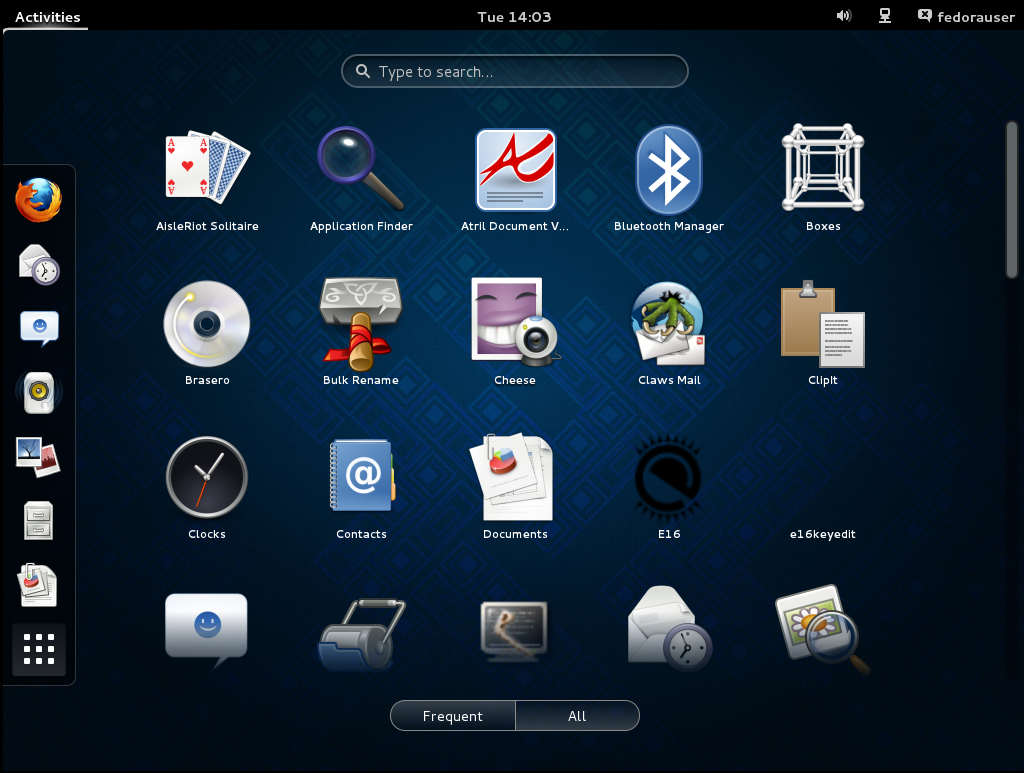
\includegraphics[scale=0.3]{Imagenes/Fedora_02.png}
\end{figure}
\end{frame}
\begin{frame}
\frametitle{Escribir el nombre}
En ambos casos se abrirá una ventana de búsqueda en donde anotaremos el nombre de nuestra aplicación: \textocolor{cadmiumgreen}{Anaconda}, para luego presionar Enter.
\end{frame}
\begin{frame}
\frametitle{Anaconda Navigator}
Tendremos disponible la suite \textocolor{cobalt}{Anaconda Navigator}.
\end{frame}
\begin{frame}
\frametitle{Anaconda Navigator}
\begin{figure}
    \centering
    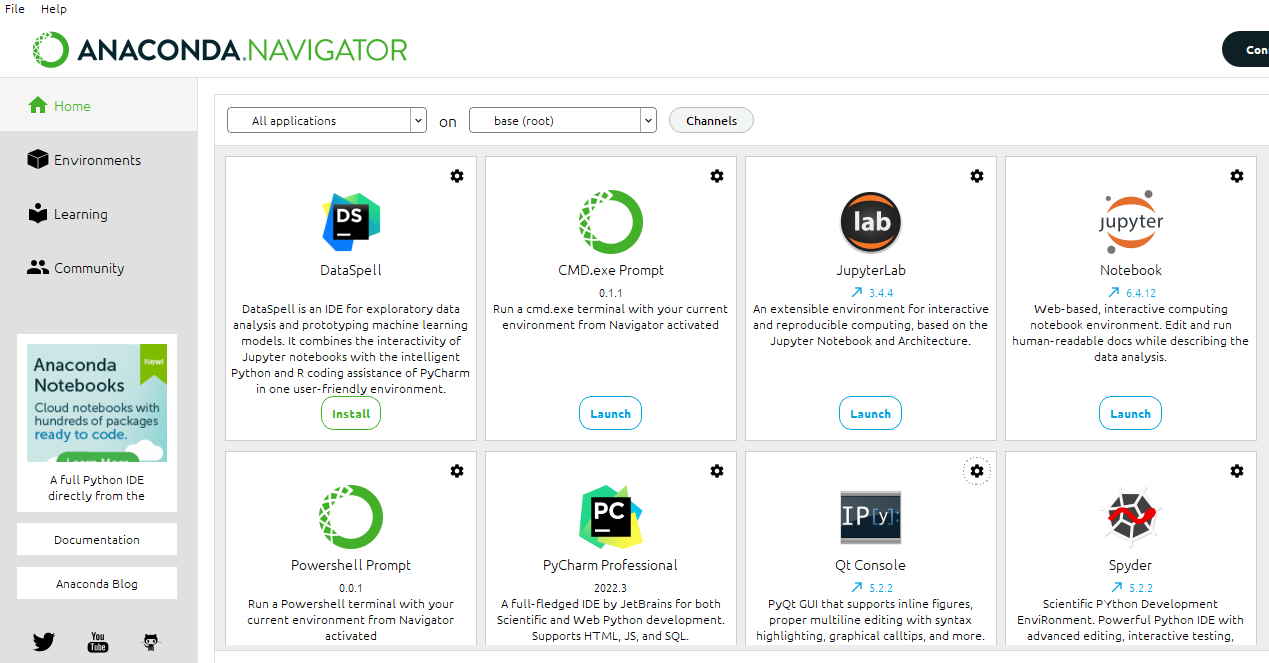
\includegraphics[scale=0.35]{Imagenes/Anaconda_01.png}
\end{figure}
\end{frame}
\begin{frame}
\frametitle{Programas disponibles}
En Anaconda Navigator tendremos disponibles:
\pause
\setbeamercolor{item projected}{bg=lava,fg=white}
\setbeamertemplate{enumerate items}{%
\usebeamercolor[bg]{item projected}%
\raisebox{1.5pt}{\colorbox{bg}{\color{fg}\footnotesize\insertenumlabel}}%
}
\begin{enumerate}[<+->]
\item \textocolor{ao}{jupyter}.
\item \textocolor{red}{Qt Console}.
\item \textocolor{byzantine}{Spyder}.
\end{enumerate}
\end{frame}
\begin{frame}
\frametitle{Qt Console}
Seleccionamos \textocolor{red}{Qt Console} para iniciar esta parte de repaso con python.
\end{frame}
\begin{frame}
\frametitle{Qt Console}
\begin{figure}
    \centering
    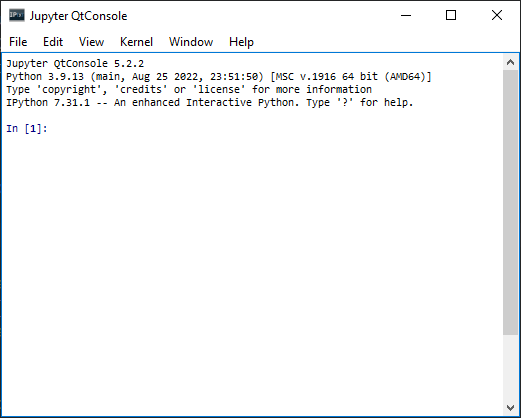
\includegraphics[scale=0.65]{Imagenes/Anaconda_02.png}
\end{figure}
\end{frame}

\section{python como una calculadora}
\frame{\tableofcontents[currentsection, hideothersubsections]}
\subsection{Operadores aritméticos}

\begin{frame}
\frametitle{\python{} como calculadora}
Una vez abierta la sesión en \python, podemos aprovechar al máximo este lenguaje: \pause para familiarizarnos con su uso, veamos la manera de usar python como una calculadora, sólo hay que ir escribiendo las operaciones en la línea de comandos.
\end{frame}

\begin{frame}[fragile]
\frametitle{Algunas operaciones}
Podemos hacer una suma:
\\
\bigskip
\textcolor{ao}{\texttt{In[1]: }} \verb|3 + 200| \\
\pause
\textcolor{red}{\texttt{Out[1]: }} \verb|203|
\end{frame}
\begin{frame}[fragile]
\frametitle{Identificador en la línea de comandos}
Nótese que en cada línea tendremos un \enquote{prompt} que nos indica la \emph{entrada}:
\\
\bigskip
\textcolor{ao}{\texttt{In[1]: }}
\pause
\\
\bigskip
y se le asigna un número consecutivo.
\end{frame}
\begin{frame}[fragile]
\frametitle{Identificador en la línea de comandos}
Dependiendo de la tarea que se ejecute, podemos tener una línea de \emph{salida} con el mismo número:
\\
\bigskip
\textcolor{red}{\texttt{Out[1]: }}
\\
\bigskip
\pause
En ciertas tareas, no se presentará esa línea de salida, sino que se mostrará una nueva línea de entrada, con su número consecutivo.
\end{frame}
\begin{frame}[fragile]
\frametitle{División entre números enteros}
Como estilo de escritura hay que dejar un espacio en blanco entre los valores y el operador que utilizemos:
\\
\bigskip
\textcolor{ao}{\texttt{In[2]: }} \verb|30 / 1234| \\
\pause
\textcolor{red}{\texttt{Out[2]: }} \verb|0.024311183144246355|
\end{frame}
\begin{frame}[fragile]
\frametitle{División entre números de punto flotante}
\bigskip
\textcolor{ao}{\texttt{In[3]: }} \verb| 3.0 / 4.0| \\
\pause
\textcolor{red}{\texttt{Out[3]: }} \verb| 0.75|
\\
\bigskip
\pause
Los números de punto flotante, llevan un punto decimal.
\end{frame}
\begin{frame}[fragile]
\frametitle{División entera}
La división entera devuelve el cociente sin decimales:
\\
\bigskip
\textcolor{ao}{\texttt{In[4]: }} \verb|30 // 7| \\
\pause
\textcolor{red}{\texttt{Out[4]: }} \verb| 4|
\end{frame}
\begin{frame}[fragile]
\frametitle{División entera}
Otro ejemplo de división entera:
\\
\bigskip
\textcolor{ao}{\texttt{In[5]: }} \verb|4 // 3| \\
\pause
\textcolor{red}{\texttt{Out[5]: }} \verb| 1|
\end{frame}
\begin{frame}[fragile]
\frametitle{Potenciación}
Cuando queremos elevar un número (base) a un exponente (potencia), hacemos:
\\
\bigskip
\textcolor{ao}{\texttt{In[6]: }} \verb|2**3| \\
\pause
\textcolor{red}{\texttt{Out[6]: }} \verb| 8|
\end{frame}
\begin{frame}[fragile]
\frametitle{Resta entre dos números}
Podemos restar dos números:
\\
\bigskip
\textcolor{ao}{\texttt{In[7]: }} \verb|1234 - 678| \\
\pause
\textcolor{red}{\texttt{Out[7]: }} \verb| 556|
\end{frame}
\begin{frame}[fragile]
\frametitle{El módulo de dos números}
Una operación común en programación es obtener el módulo de dos números:
\\
\bigskip
\textcolor{ao}{\texttt{In[5]: }} \verb|17 % 3| \\
\pause
\textcolor{red}{\texttt{Out[5]: }} \verb| 2|
\\
\bigskip
\pause
Como podrás revisar, nos devuelve el residuo del cociente entre los números.
\end{frame}
\begin{frame}[fragile]
\frametitle{Combinación de operadores artiméticos}
En ocasiones tendremos que realizar en una misma línea de código, varias operaciones artiméticas:
\\
\bigskip
\textcolor{ao}{\texttt{In[8]: }} \verb| 5.0 / 10 * 2 + 5| \\
\pause
\textcolor{red}{\texttt{Out[8]: }} \verb| 6.0|
\pause
\\
\bigskip
\textbf{¿por qué obtenemos este resultado?}
\\
\bigskip
\pause
\textbf{¿en qué orden realizaste las operaciones?}
\end{frame}
\begin{frame}[fragile]
\frametitle{Uso de paréntesis}
El resultado cambia cuando agrupamos con paréntesis:
\\
\bigskip
\textcolor{ao}{\texttt{In[9]: }} \verb| 5.0 / (10 * 2 + 5)| \\
\pause
\textcolor{red}{\texttt{Out[9]: }} \verb| 0.2|
\pause
\\
\bigskip
Como podemos ver, el uso de paréntesis en las expresiones tiene una particular importancia sobre el orden en que se evalúan las expresiones.
\end{frame}
\begin{frame}
\frametitle{Sobre el uso de paréntesis}
\setbeamercolor{item projected}{bg=coolblack,fg=columbiablue}
\setbeamertemplate{enumerate items}{%
\usebeamercolor[bg]{item projected}%
\raisebox{1.5pt}{\colorbox{bg}{\color{fg}\footnotesize\insertenumlabel}}%
}
\begin{enumerate}[<+->]
\item Las expresiones contenidas dentro de pares de paréntesis se evalúan primero.
\item En el caso de expresiones con paréntesis anidados, los operadores en el par de paréntesis más interno se evalúan primero.
\end{enumerate}
\end{frame}
\begin{frame}
\frametitle{Precedencia de los operadores artiméticos}
En programación es muy importante tomar en cuenta el orden y sentido en que se realizan las operaciones aritméticas, ya que siguen una serie de reglas.
\\
\bigskip
\pause
Las reglas se indican a continuación:
\end{frame}
\begin{frame}
\frametitle{Precedencia de los operadores aritméticos}
\setbeamercolor{item projected}{bg=coolblack,fg=columbiablue}
\setbeamertemplate{enumerate items}{%
\usebeamercolor[bg]{item projected}%
\raisebox{1.5pt}{\colorbox{bg}{\color{fg}\footnotesize\insertenumlabel}}%
}
\begin{enumerate}[<+->]
\item La multiplicación, división y módulo son las siguientes en ser evaluadas. 
\item Si una expresión contiene muchas multiplicaciones, divisiones u operaciones de módulo, los operadores se evaláun de izquierda a derecha.
\seti
\end{enumerate}
\end{frame}
\begin{frame}
\frametitle{Precedencia de los operadores aritméticos}
\setbeamercolor{item projected}{bg=coolblack,fg=columbiablue}
\setbeamertemplate{enumerate items}{%
\usebeamercolor[bg]{item projected}%
\raisebox{1.5pt}{\colorbox{bg}{\color{fg}\footnotesize\insertenumlabel}}%
}
\begin{enumerate}[<+->]
\conti
\item La suma y resta son las operaciones que se evalúan al último. 
\item Si una expresión contiene muchas operaciones de suma y resta, los operadores se evalúan de izquierda a derecha.
\item La suma y resta tienen el mismo nivel de precedencia.
\end{enumerate}
\end{frame}

\subsection{Operadores relacionales}

\begin{frame}
\frametitle{Operadores relacionales}
Cuando se comparan dos (o más expresiones) mediante un operador, el tipo de dato que se devuelve es lógico: \textoazul{\textbf{True}} o \textcolor{red}{\textbf{False}}, que también tienen una representación de tipo numérico:
\pause
\begin{itemize}
\item[\ding{212}] \textoazul{\textbf{True}} = $1$
\item[\ding{212}] \textcolor{red}{\textbf{False}} = $0$
\end{itemize}
\end{frame}
\begin{frame}[fragile]
\frametitle{Operaciones aritméticas y relacionales}
Podemos extender el manejo con \python, al combinar las operaciones aritméticas y relacionales, nótese que siempre tendremos como respuesta un valor booleano:
\\
\bigskip
\textcolor{ao}{\texttt{In[10]: }} \verb| 1 + 2 > 7 - 3| \\
\pause
\textcolor{red}{\texttt{Out[10]: }} \verb| False|
\end{frame}
\begin{frame}[fragile]
\frametitle{Operaciones aritméticas y relacionales}
Otro ejemplo en donde ahora tenemos dos expresiones relacionales:
\\
\bigskip
\textcolor{ao}{\texttt{In[11]: }} \verb| 1 < 2 < 3| \\
\pause
\textcolor{red}{\texttt{Out[11]: }} \verb| True|
\end{frame}
\begin{frame}[fragile]
\frametitle{El operador de comparación de igualdad}
El doble signo igual ($==$) es el operador de igualdad, a diferencia del operador $=$ que es el operador de asignación.
\\[1em]
\textcolor{ao}{\texttt{In[12]: }} \verb| 1 > 2 == 2 < 3| \\
\pause
\textcolor{red}{\texttt{In[12]: }} \verb| False|
\end{frame}
\begin{frame}[fragile]
\frametitle{Combinación de expresiones}
\textcolor{ao}{\texttt{In[13]: }} \verb| 3 > 4 < 5| \\
\pause
\textcolor{red}{\texttt{In[13]: }} \verb| False|
\\
\bigskip
\pause
\textcolor{ao}{\texttt{In[14]: }} \verb| 1.0 / 3 < 0.3333| \\
\pause
\textcolor{red}{\texttt{In[14]: }} \verb| False|
\\
\bigskip
\pause
\textcolor{ao}{\texttt{In[15]: }} \verb| 5.0 / 3 >= 11 /7.0| \\
\pause
\textcolor{red}{\texttt{In[15]: }} \verb| True|
\end{frame}
\begin{frame}[fragile]
\frametitle{Combinación de expresiones}
Las expresiones se pueden complicar cada vez más, por lo que hay que mantener atención al momento de escribirlas.
\\
\bigskip
\pause
Se recomienda siempre el uso de parentésis para identificar las operaciones que se vayan a realizar.
\end{frame}
\begin{frame}
\frametitle{Tabla de operadores relacionales}
\begin{table}
\fontsize{12}{12}\selectfont
\begin{tabular}{| c | l | c | c |}
\hline
Operador & Operación & Ejemplo & Resultado\\ \hline
$==$ & Igual a & $4==5$ & \textcolor{red}{\texttt{False}} \\ \hline
$!=$ & Diferente & $2!=3$ & \textoazul{\texttt{True}} \\ \hline
$<$ & Menor que & $ 10<4$  & \textcolor{red}{\texttt{False}} \\ \hline
$>$ & Mayor que & $5>-4$ & \textoazul{\texttt{True}} \\ \hline
$<=$ & Menor o igual & $7<=7$ & \textoazul{\texttt{True}} \\ \hline
$>=$ & Mayor o igual & $3.5 >= 10$ & \textcolor{red}{\texttt{False}} \\ \hline
\end{tabular}
\end{table}
\end{frame}

\subsection{Operadores booleanos}

\begin{frame}
\frametitle{Operadores booleanos}
En \python{} existen tres operadores booleanos:
\setbeamercolor{item projected}{bg=cobalt,fg=white}
\setbeamertemplate{enumerate items}{%
\usebeamercolor[bg]{item projected}%
\raisebox{1.5pt}{\colorbox{bg}{\color{fg}\footnotesize\insertenumlabel}}%
}
\begin{enumerate}[<+->]
\item \azulfuerte{and}
\item \azulfuerte{or}
\item \azulfuerte{not}
\end{enumerate}
\pause
Estos operadores comparan valores booleanos, el resultado de ésta comparación se expresa en un valor booleano.
\end{frame}
\begin{frame}[fragile]
\frametitle{El operador booleano \texttt{and}}
Cuando comparamos dos expresiones con el operador booleano \azulfuerte{and}, tendremos de respuesta un valor \textoazul{True}, siempre y cuando ambas expresiones sean verdaderas:
\\
\bigskip
\pause
\textcolor{ao}{\texttt{In[18]: }} \verb| (4 < 5) and (5 < 6)| \\
\pause
\textcolor{red}{\texttt{Out[18]: }} \verb| True|
\end{frame}
\begin{frame}[fragile]
\frametitle{El operador booleano \texttt{and}}
En caso de que una de las expresiones sea \textcolor{red}{False} (incluso las dos expresiones), al momento de compararlas con el operador booleano \azulfuerte{and}, el resultado que se devuelve es \textcolor{red}{False}:
\\
\bigskip
\pause
\textcolor{ao}{\texttt{In[19]: }} \verb| (4 < 5) and (9 < 6)| \\
\pause
\textcolor{red}{\texttt{Out[19]: }} \verb| False|
\end{frame}
\begin{frame}[fragile]
\frametitle{El operador booleano \texttt{or}}
El operador booleano \azulfuerte{or} devuelve un valor \textoazul{True}, cuando una de las expresiones es verdadera (incluso ambas):
\\
\bigskip
\pause
\textcolor{ao}{\texttt{In[20]: }} \verb| (1==2) or (2 == 2)| \\
\pause
\textcolor{red}{\texttt{Out[20]: }} \verb| True|
\end{frame}
\begin{frame}[fragile]
\frametitle{El operador booleano \texttt{or}}
Si las expresiones que se comparan con el operador booleano \azulfuerte{or} son ambas falsas, se tendrá como respuesta un valor \textcolor{red}{False}:
\\
\bigskip
\pause
\textcolor{ao}{\texttt{In[21]: }} \verb| (1 > 2) or (8 == 2)| \\
\pause
\textcolor{red}{\texttt{Out[21]: }} \verb| False|
\end{frame}
\begin{frame}[fragile]
\frametitle{El operador booleano \texttt{not}}
El operador booleano \azulfuerte{not} \enquote{niega} (invierte) el valor booleano de la expresión que evalúa:
\\
\bigskip
\pause
\textcolor{ao}{\texttt{In[22]: }} \verb| not(True)| \\
\pause
\textcolor{red}{\texttt{Out[22]: }} \verb| False|
\end{frame}
\begin{frame}[fragile]
\frametitle{El operador booleano \texttt{not}}
Podemos ocupar una expresión más elaborada en la que anticipamos el resultado y entonces se ocupa el operador \azulfuerte{not}, para negar el resultado:
\\
\bigskip
\pause
{\fontsize{12}{12}\selectfont
\textcolor{ao}{\texttt{In[23]: }} \verb|((2 + 2) == 4) and (not((2 + 2) == 5))|} \\
\pause
\textcolor{red}{\texttt{Out[23]: }} \verb| True|
\end{frame}
\begin{frame}[fragile]
\frametitle{Posibles errores al introducir valores/operaciones}
Será muy común al inicio encontrar errores cuando se teclean las instrucciones en el código, por lo que hay que tomar en cuenta los avisos que nos devuelve \python:
\\
\bigskip
\pause
\textcolor{ao}{\texttt{In[16]: }} \verb| 5 + | \\
\pause
\verb| File "<stdin>", line 1| \\
\verb|      5 +  | \\
\verb|         ^| \\
\textcolor{red}{\texttt{SyntaxError:}}\verb| invalid syntax|
\end{frame}
\begin{frame}
\frametitle{Posibles errores}
Lo que nos indica que se presenta un error, en este caso, un \textbf{error de sintaxis}.
\\
\bigskip
\pause
Encontraremos en python distintos tipos de error que se generan en particulares situaciones. \pause Más adelante, mostraremos la manera en la que podemos manejar esos errores para evitar que el programa se detenga.
\end{frame}
\begin{frame}[fragile]
\frametitle{Posibles errores al introducir valores/operaciones}
\textcolor{ao}{\texttt{In[17]: }} \verb| 42 + 5 + * 2 | \\
\pause
\verb| File "<stdin>", line 1| \\
\verb|   42 + 5 + * 2 | \\
\verb|            ^| \\
\textcolor{red}{\texttt{SyntaxError:}}\verb| invalid syntax|
\end{frame}
\begin{frame}[fragile]
\frametitle{Posibles errores al introducir valores/operaciones}
\textcolor{ao}{\texttt{In[17]: }} \verb| 3 / 0 | \\
\pause
{\fontsize{12}{12}\selectfont
\verb|ZeroDivisionError | \\
\verb|Traceback (most recent call last)| \\
\verb|<ipython-input-1-e1965806ec03> in <module>| \\
\verb|----> 1 3 / 0| \\
\textcolor{red}{\texttt{ZeroDivisionError:}}\verb| division by zero|}
\end{frame}
    

\section{Las variables en python}
\frame{\tableofcontents[currentsection, hideothersubsections]}
\subsection{Tipos de variables}

\begin{frame}
\frametitle{¿Qué es una variable?}
Una variable es una ubicación de memoria reservada para almacenar valores que se modifican durante la ejecución de un programa.
\\
\bigskip
\pause
Las variables en python no necesitan una declaración explícita para reservar el espacio en memoria. La declaración ocurre automáticamente cuando se asigna un valor a una variable.
\end{frame}
\begin{frame}[fragile]
\frametitle{Declarando variables}
Establecemos una variable de la siguiente forma:
\\[1em]
\pause
\verb| nombre_variable = valor_inicial |
\\
\bigskip
Nótese que la asignación de un valor a una variable se hace mediante el operador $=$, ya vimos que una comparación entre valores se hace con el doble igual ($==$).
\end{frame}
\begin{frame}[fragile]
\frametitle{Escribiendo variables}
Se recomienda utilizar un nombre corto asociado a lo que va a contener la variable, se puede extender el nombre de la misma, usando el guión bajo, nunca espacios en blanco.
\\
\bigskip
\pause
\verb| distancia = 145.5 | \\
\verb| tiempo_segundos = 60 | \\
\verb| nombre_catalogo = "NGC1952" |
\end{frame}
\begin{frame}[fragile]
\frametitle{Valores constantes}
Cuando se tiene el caso particular de una variable que no se modifica, entonces tenemos una constante.
\pause
\begin{eqnarray*}
g &= 9.81 \\
\mbox{ANGULO} &= 27
\end{eqnarray*}
\pause 
Se recomienda que el nombre de las constantes se anote en mayúsculas.
\end{frame}

\section{Tipos de datos}
\frame{\tableofcontents[currentsection, hideothersubsections]}
\subsection{Los tipos de datos}

\begin{frame}
\frametitle{¿Qué es un tipo de dato}
En python como en la mayoría de lenguajes de programación, los tipos de datos definen un conjunto de valores con características y propiedades particulares.
\\
\bigskip
\pause
Cuando asignamos un valor a una variable, se define ese conjunto de valores que puede tomar así como las operaciones que están permitidas.
\end{frame}

\subsection{Tipos numéricos}

\begin{frame}
\frametitle{Los tipos numéricos en \python}
Los tipos de datos numéricos que se manejan en python son los siguientes:
\setbeamercolor{item projected}{bg=darkblue,fg=daffodil}
\setbeamertemplate{enumerate items}{%
\usebeamercolor[bg]{item projected}%
\raisebox{1.5pt}{\colorbox{bg}{\color{fg}\footnotesize\insertenumlabel}}%
}
\begin{enumerate}[<+->]
\item Enteros.
\item Punto flotante.
\item Complejos.
\end{enumerate}
\end{frame}
\begin{frame}
\frametitle{Tipo entero}
Los números enteros son aquellos que no tienen decimales, tanto positivos como negativos (además del cero).
\\
\bigskip
\pause
En python este tipo de dato se representa como $\texttt{int}$ (de integer, entero).
\end{frame}
\begin{frame}[fragile]
\frametitle{Ejemplo de datos enteros}
\begin{lstlisting}[caption=Ejecuta el código y revisa el resultado]
a = 10
b = -6
print(a - b)
\end{lstlisting}
\end{frame}
\begin{frame}
\frametitle{Otras representaciones}
Los números enteros también se pueden representar en otros sistemas:
\pause
\setbeamercolor{item projected}{bg=lava,fg=laserlemon}
\setbeamertemplate{enumerate items}{%
\usebeamercolor[bg]{item projected}%
\raisebox{1.5pt}{\colorbox{bg}{\color{fg}\footnotesize\insertenumlabel}}%
}
\begin{enumerate}[<+->]
\item Binario: se utiliza el prefijo 0b a una secuencia de dígitos en binario (0 y 1).
\item Octal: se utiliza el prefijo 0o a una secuencia de dígitos octales (del 0 al 7).
\item Hexadecimal: se utiliza el prefijo 0x a una secuencia de dígitos en hexadecimal (del 0 al 9 y de la A la F).
\end{enumerate}
\end{frame}
\begin{frame}[fragile]
\frametitle{Escribiendo el valor de $10$}
\begin{lstlisting}[caption=Representando otros formatos]
diez = 10
diez_binario = 0b1010
diez_oct = 0o12
diez_hex =0xa
\end{lstlisting}
\end{frame}
\begin{frame}[fragile]
\frametitle{Presentando el valor de $10$}
\begin{lstlisting}[caption=Ejecuta el código para revisar el resultado]
print(10)
print(diez_binario)
print(diez_oct)
print(diez_hex)
\end{lstlisting}
\end{frame}

\subsection{Tipos de datos de punto flotante}

\begin{frame}
\frametitle{Números de punto flotante}
Los números reales son los que tienen decimales. En python se expresan mediante el tipo $\texttt{float}$.
\\
\bigskip
\pause
Se implementa su tipo $\texttt{float}$ utilizando 64 bits, en concreto se sigue el estándar \textbf{IEEE 754}: 1 bit para el signo, 11 para el exponente, y 52 para la mantisa. En el Tema 1, ampliaremos esta información.
\end{frame}
\begin{frame}
\frametitle{Números de punto flotante}
Recordemos que cada valor asignado a una variable ocupa un espacio de memoria en la computadora, \pause al principio puede parecer que tendremos bastante espacio de sobra para nuestras operaciones.
\end{frame}
\begin{frame}
\frametitle{Números de punto flotante}
Pero conforme avancemos en el contenido del curso, los recursos de memoria serán críticos para determinar si nuestra computadora tendrá la capacidad de soportar las tareas que necesitemos.
\end{frame}
\begin{frame}[fragile]
\frametitle{Manejando números de punto flotante}
\begin{lstlisting}[caption=Ejemplo con datos de punto flotante]
velocidad = 10.37

print(velocidad**2)
\end{lstlisting}
\end{frame}
\begin{frame}[fragile]
\frametitle{Revisa con cuidado el siguiente ejemplo}
\begin{lstlisting}[caption=Escribe y ejecute el siguiente código]
1.1 + 2.2
\end{lstlisting}
\pause
Ups! \textbf{¿qué pasó? ¿de donde sale ese valor} $\ldots 3$ al final del renglón? \pause Cuando revisemos el tema de artimética de punto flotante, tendremos la respuesta a estas dos preguntas.
\end{frame}

\subsection{Tipos de datos complejos}

\begin{frame}
\frametitle{Números complejos}
Un número complejo consiste en un par ordenado de números reales de coma flotante denotados por: \pause $ x + y \, j$ donde $x$ e $y$ son números reales, \pause mientras que $y \, j$ es la unidad imaginaria.
\\
\bigskip
\pause
Un valor complejo es de tipo $\texttt{complex}$.
\end{frame}
\begin{frame}
\frametitle{Números complejos}    
Nótese que $j$ representa $\sqrt{-1}$, no se ocupa $i$ ya que como veremos, esa letra se presenta más en las estructuras de control.
\\
\bigskip
\pause
Este tipo de dato sigue el álgebra de los números complejos.
\end{frame}
\begin{frame}[fragile]
\frametitle{Ejemplo con números complejos}
\begin{lstlisting}[caption=Ejercicio con números complejos]
a = 3 + 4j
b = 5 - 2j

print(a + b)
print(a * b)
\end{lstlisting}
\end{frame}
\begin{frame}[fragile]
\frametitle{La parte real e imaginaria de un complejo}
Podemos recuperar la parte real y la parte imaginaria de un número complejo:
\pause
\begin{lstlisting}[caption=Parte real y compleja]
print(a.real)
print(a.imag)
\end{lstlisting}
\end{frame}
\begin{frame}[fragile]
\frametitle{Operaciones entre distintos tipos de números}
Es posible realizar operaciones artiméticas con tipos numéricos distintos, el resultado corresponderá al mismo tipo de dato de mayor valor:
\pause
\begin{lstlisting}[caption=Ejemplos de operaciones entre tipos de datos numéricos]
print(3.14 + 10 - 2j)
print()
print(10 + 2.3)
\end{lstlisting}
\end{frame}

\section{Cadenas}
\frame{\tableofcontents[currentsection, hideothersubsections]}
\subsection{Definición}

\begin{frame}
\frametitle{¿Qué son las cadenas?}
Las cadenas en \python{} se identifican como un conjunto o secuencia de caracteres representados en las comillas.
\\
\bigskip
\pause
A una cadena se le asocia el tipo de dato $\texttt{str}$ (de \emph{string}).
\end{frame}
\begin{frame}[fragile]
\frametitle{Escribiendo una cadena}
Se permite cualquier par de 'comillas simples' o comillas \enquote{dobles}.
\pause
\begin{lstlisting}[caption=Escribiendo cadenas de texto]
print("Hola Mundo!")
print()
print('La velocidad de la luz es finita.')
print()
print('No choqué, "me chocaron!"')
print()
print('El balón es \'casi\' esférico.')
\end{lstlisting}
\end{frame}

\subsection{Manejo de las cadenas}

\begin{frame}
\frametitle{Ocupando las cadenas de texto}
El tipo de dato $\texttt{str}$ contiene un conjunto muy amplio de funciones que nos permiten manipular a una cadena de la forma en que nos interese.
\\
\bigskip
\pause
En el desarrollo del curso, veremos algunas de esas funciones que serán de utilidad.
\end{frame}
\begin{frame}
\frametitle{Extendiendo la información}
Para conocer más a detalle las funciones que se pueden aplicar a una cadena de texto, pueden consultar la \underline{\href{https://docs.python.org/es/3/library/string.html}{documentación oficial}} en el sitio web de \python.
\end{frame}
\begin{frame}[fragile]
\frametitle{Uniendo dos cadenas}
Revisemos el siguiente ejemplo:
\pause
\begin{lstlisting}[caption=Concatenación de cadenas]
cadena1 = "Facultad de Ciencias,"
cadena2 = "UNAM."
print(cadena1 + cadena2)
\end{lstlisting}
\end{frame}
\begin{frame}
\frametitle{Uniendo dos cadenas}
En el ejemplo anterior hemos utilizado el operador de \textoazul{concatenación} entre cadenas, \pause pero vemos que el contenido de las mismas, queda sin espacio:
\begin{align*}
\mbox{Facultad de Ciencias,UNAM}
\end{align*}
\end{frame}
\begin{frame}[fragile]
\frametitle{Ajustando el espacio}
Por ello hay que incluir un espacio en blanco a modo de separador:
\pause
\begin{lstlisting}[caption=Ajustando el espacio entre las cadenas,]
print(cadena1 + " " + cadena2)
\end{lstlisting}
\end{frame}

\subsection{Cadenas e índices}

\begin{frame}[fragile]
\frametitle{Nueva cadena}
Indiquemos una nueva cadena:
\begin{lstlisting}[caption=Nueva cadena]
cadena = 'Ciencias'
print(cadena)
\end{lstlisting}
\end{frame}
\begin{frame}
\frametitle{Los índices en una cadena}
La manera en la que se almacena una variable de tipo cadena en python es la siguiente:
\pause
\begin{figure}
    \centering
    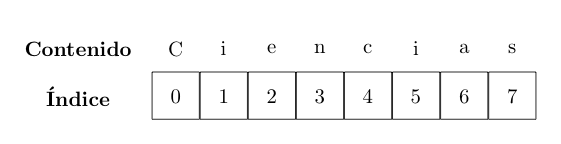
\includegraphics[scale=1]{Imagenes/variablecadena01.png}
\end{figure}
\pause
Cada caracter se almacena en un espacio que se identifica mediante un índice, en python \textbf{los índices comienzan en cero}.
\end{frame}
\begin{frame}[fragile]
\frametitle{Manejando los índices}
Manejando los índices de una cadena podemos recuperar el contenido de la misma, para ello indicamos entre corchetes el valor del índice que nos interesa:
\pause
\begin{lstlisting}[caption=Usando índices en una cadena]
print(cadena[0])
print(cadena[1])
print(cadena[2])
\end{lstlisting}
\end{frame}
\begin{frame}[fragile]
\frametitle{Manejando los índices}
Es posible ocupar valores negativos para los índices:
\pause
\begin{lstlisting}[caption=Usando índices negativos]
print(cadena[7])
print()
print(cadena[-1])
\end{lstlisting}
\pause
Vemos que se recupera el contenido de la cadena mediante el índice $7$ o $-1$, es decir, el último elemento de la cadena.
\end{frame}
\begin{frame}[fragile]
\frametitle{Manejando los índices}
Podemos hacer lo mismo para recuperar el primer elemento, como se ve en dos celdas anteriores:
\pause
\begin{lstlisting}[caption=Usando índices negativos y el primer elemento]
print(cadena[-8])
print()
print(cadena[0])
\end{lstlisting}
\end{frame}
\begin{frame}
\frametitle{Partiendo una cadena}
En ocasiones será necesario recuperar no solo un elemento de la cadena, sino una parte con varios elementos, para ello se ocupa el \emph{slicing} (rebanado), dentro de los corchetes debemos de ocupar la sintaxis:
\pause
\begin{align*}
[ \, \mbox{índice inicial} \, : \, \mbox{índice final} \, ]
\end{align*}
\end{frame}
\begin{frame}[fragile]
\frametitle{Seleccionando parte de una cadena}
Veamos como hacemos el \emph{slicing} en nuestra cadena:
\pause
\begin{lstlisting}[caption=Haciendo una selección dentro de la cadena]
print(cadena[2:4])
print()
print(cadena[2:])
print()
print(cadena[:8])
\end{lstlisting}
\end{frame}
\begin{frame}
\frametitle{Lo que se recupera con el slicing}
Del ejemplo anterior se recupera:
\setbeamercolor{item projected}{bg=lava,fg=white}
\setbeamertemplate{enumerate items}{%
\usebeamercolor[bg]{item projected}%
\raisebox{1.5pt}{\colorbox{bg}{\color{fg}\footnotesize\insertenumlabel}}%
}
\begin{enumerate}[<+->]
\item Línea 1: Los caracteres del índice 2, 3 pero no el 4.
\item Línea 3: Los caracteres desde el índice 2 hasta el final de la cadena.
\item Línea 5: Recupera toda la cadena
\end{enumerate}
\end{frame}
\begin{frame}[fragile]
\frametitle{Repitiendo el contenido de una cadena}
Cuando tenemos una cadena, es posible repetir la misma un determinado número de veces, para ello se utiliza el \textoazul{operador de repetición} $*$:
\pause
\begin{lstlisting}[caption=El operador de repetición de cadenas]
print(cadena*2)
\end{lstlisting}
\pause
Nótese que no hay un espacio entre el contenido de la cadena, ya que así se definió. \pause El operador de repetición cumple la tarea de mostrar la cadena el número de veces que se indica.
\end{frame}
\begin{frame}[fragile]
\frametitle{Usos del operador de repetición}
Este operador de repetición es de mucha utilidad si queremos simplificar una tarea que nos apoye para visualizar un resultado:
\pause
\begin{lstlisting}[caption=Ejemplo de repetición de un caracter]
print('Temperatura \t Presión')
print('-' * 25)
\end{lstlisting}
\pause
En la primera línea se ocupa un \textoazul{tabulador}, que es una secuencia de escape.
\end{frame}
\begin{frame}
\frametitle{Las secuencias de escape en python}
Una secuencia de escape no es propiamente un texto que se visualice, más bien, es una combinación de una barra invertida $\backslash$ y otra letra que permite dentro de una cadena de texto:
\setbeamercolor{item projected}{bg=darkgreen,fg=laserlemon}
\setbeamertemplate{enumerate items}{%
\usebeamercolor[bg]{item projected}%
\raisebox{1.5pt}{\colorbox{bg}{\color{fg}\footnotesize\insertenumlabel}}%
}
\begin{enumerate}[<+->]
\item $\backslash \mbox{t}$ aplica un tabulador.
\item $\backslash \mbox{n}$ un salto de línea.
\item $\backslash \backslash$ imprimir una barra invertida.
\end{enumerate}
\end{frame}
\begin{frame}[fragile]
\frametitle{Uso de caracteres de escape}
Vemos lo siguiente:
\begin{lstlisting}[caption=Algunos caracteres de escape]
print('Este texto incluye \t una tabulación')
print()
print('En una cadena podemos incluir \n un salto de línea')
print()
print('Si queremos una barra invertida \\ la podemos incluir!')
\end{lstlisting}
\end{frame}
\begin{frame}[fragile]
\frametitle{Extendiendo la lectura de resultados}
Veremos que es posible combinar dentro de la función \textbf{print ( )} cadenas y valores:
\pause
\begin{lstlisting}[caption=Combinación de cadenas y valores]
radio = 3
pi = 3.14
area = pi * radio**2
print(area)
\end{lstlisting}
\end{frame}
\begin{frame}[fragile]
\frametitle{Modificando la salida del resultado}
Ahora veamos lo siguiente:
\begin{lstlisting}[caption=Un texto y un valor de salida]
print('El valor del área es: ', area)
\end{lstlisting}
Lo que nos facilita la lectura e interpretación del resultado.
\end{frame}
\begin{frame}[fragile]
\frametitle{Una lectura mucho más agradable}
Con el siguiente código que incluye la función \textoazul{format}, propia de las cadenas de texto, tendremos un resultado más amigable de leer:
\begin{lstlisting}[caption=Un texto y un valor de salida 2a. versión]
print('El valor del área de un círculo de radio {0:} unidades, es {1:} unidades al cuadrado'.format(radio, area))
\end{lstlisting}
Las llaves \{ $0:$ \} y \{ $1:$ \} indican el orden en que se presentarán las variables dentro de la función \emph{format}.
\end{frame}
\begin{frame}[fragile]
\frametitle{¿Concatenando cadenas y números?}
¿Qué ocurre si queremos concatenar la cadena con el valor de la variable radio?
\pause
\begin{lstlisting}[caption=Ejemplo de concatenación de cadenas y números]
print('El círculo tiene un radio de ' + radio + ' unidades.')
\end{lstlisting}
\pause
Se presenta un error que nos indica que no podemos concatenar cadenas con números.
\end{frame}
\begin{frame}[fragile]
\frametitle{Modificando el código}
Esto lo resolvemos si hacemos un cambio en la variable radio, la pasamos de un tipo de dato $\texttt{int}$ a uno de tipo $\texttt{str}$:
\pause
\begin{lstlisting}[caption=Usando función de conversión de tipo de dato]
print('El círculo tiene un radio de ' + str(radio) + ' unidades.')
\end{lstlisting}
\end{frame}
\begin{frame}
\frametitle{Manejando tipos de datos consistentes}
Este tipo de conversión le llamamos de manera lúdica: manzanas con manzanas y peras con peras, es decir, manipulamos variables que sea del mismo tipo de dato.
\end{frame}
\begin{frame}
\frametitle{Manejando tipos de datos consistentes}
Las funciones que nos permiten hacer la conversión son:
\pause
\setbeamercolor{item projected}{bg=lava,fg=white}
\setbeamertemplate{enumerate items}{%
\usebeamercolor[bg]{item projected}%
\raisebox{1.5pt}{\colorbox{bg}{\color{fg}\footnotesize\insertenumlabel}}%
}
\begin{enumerate}[<+->]
\item \texttt{str( )}: Nos devuelve la representación en una cadena de caracteres del objeto que se pasa como parámetro.
\item \texttt{int( )}: Devuelve un valor enterio a partir de un número o secuencia de caracteres.
\seti
\end{enumerate}
\end{frame}
\begin{frame}
\frametitle{Manejando tipos de datos consistentes}
\setbeamercolor{item projected}{bg=lava,fg=white}
\setbeamertemplate{enumerate items}{%
\usebeamercolor[bg]{item projected}%
\raisebox{1.5pt}{\colorbox{bg}{\color{fg}\footnotesize\insertenumlabel}}%
}
\begin{enumerate}[<+->]    
\conti 
\item \texttt{float( )}: Devuelve un valor de punto flotante a partir de un número o secuencia de caracteres.
\item \texttt{complex( )}: Devuelve un complex a partir de un número o secuencia de caracteres.
\end{enumerate}
\end{frame}
\begin{frame}[fragile]
\frametitle{Conociendo el tipo de dato}
La manera en la que podemos conocer el tipo de dato de una variable en python es muy sencilla: con la función \textoazul{type( )}, tendremos la respuesta:
\pause
\begin{lstlisting}[caption=Usando la función type()]
type("Estrella")
type(2)
type(3.14156)
type(2 + 5j)
\end{lstlisting}
\end{frame}
\end{document}